\documentclass[tikz,border=11pt]{standalone}
\usetikzlibrary{arrows.meta, positioning, calc, math}

\def\rthick{0.2} % rectangle thickness

\tikzset{
  poststyle/.style={thick, fill=blue!20},
  compstyle/.style={thick, fill=green!20},
  sendstyle/.style={thick, fill=red!20},
  recvstyle/.style={thick, fill=orange!20}
}
\newcommand{\rankcontroller}{
  % place a coordinate rx at (2, 0)
  \coordinate (ro) at (2, 0);
  \coordinate (co) at (6, 0);

  \begin{scope}[shift={(-0.0, 0)}]
    \draw[->,thick,-stealth] (0, 0) -- (0, -10);
  \end{scope}

  \begin{scope}[shift={(ro)}]
    \node[rankbox] (rx) at (0,0) {$Rank$};
    \draw[style=dotted] (rx.south) -- (0, -10);
  \end{scope}

  \begin{scope}[shift={(co)}]
    \node[rankbox] (ry) at (0,0) {$Controller$};
    \draw[style=dotted] (ry.south) -- (0, -10);
  \end{scope}
}

\begin{document}
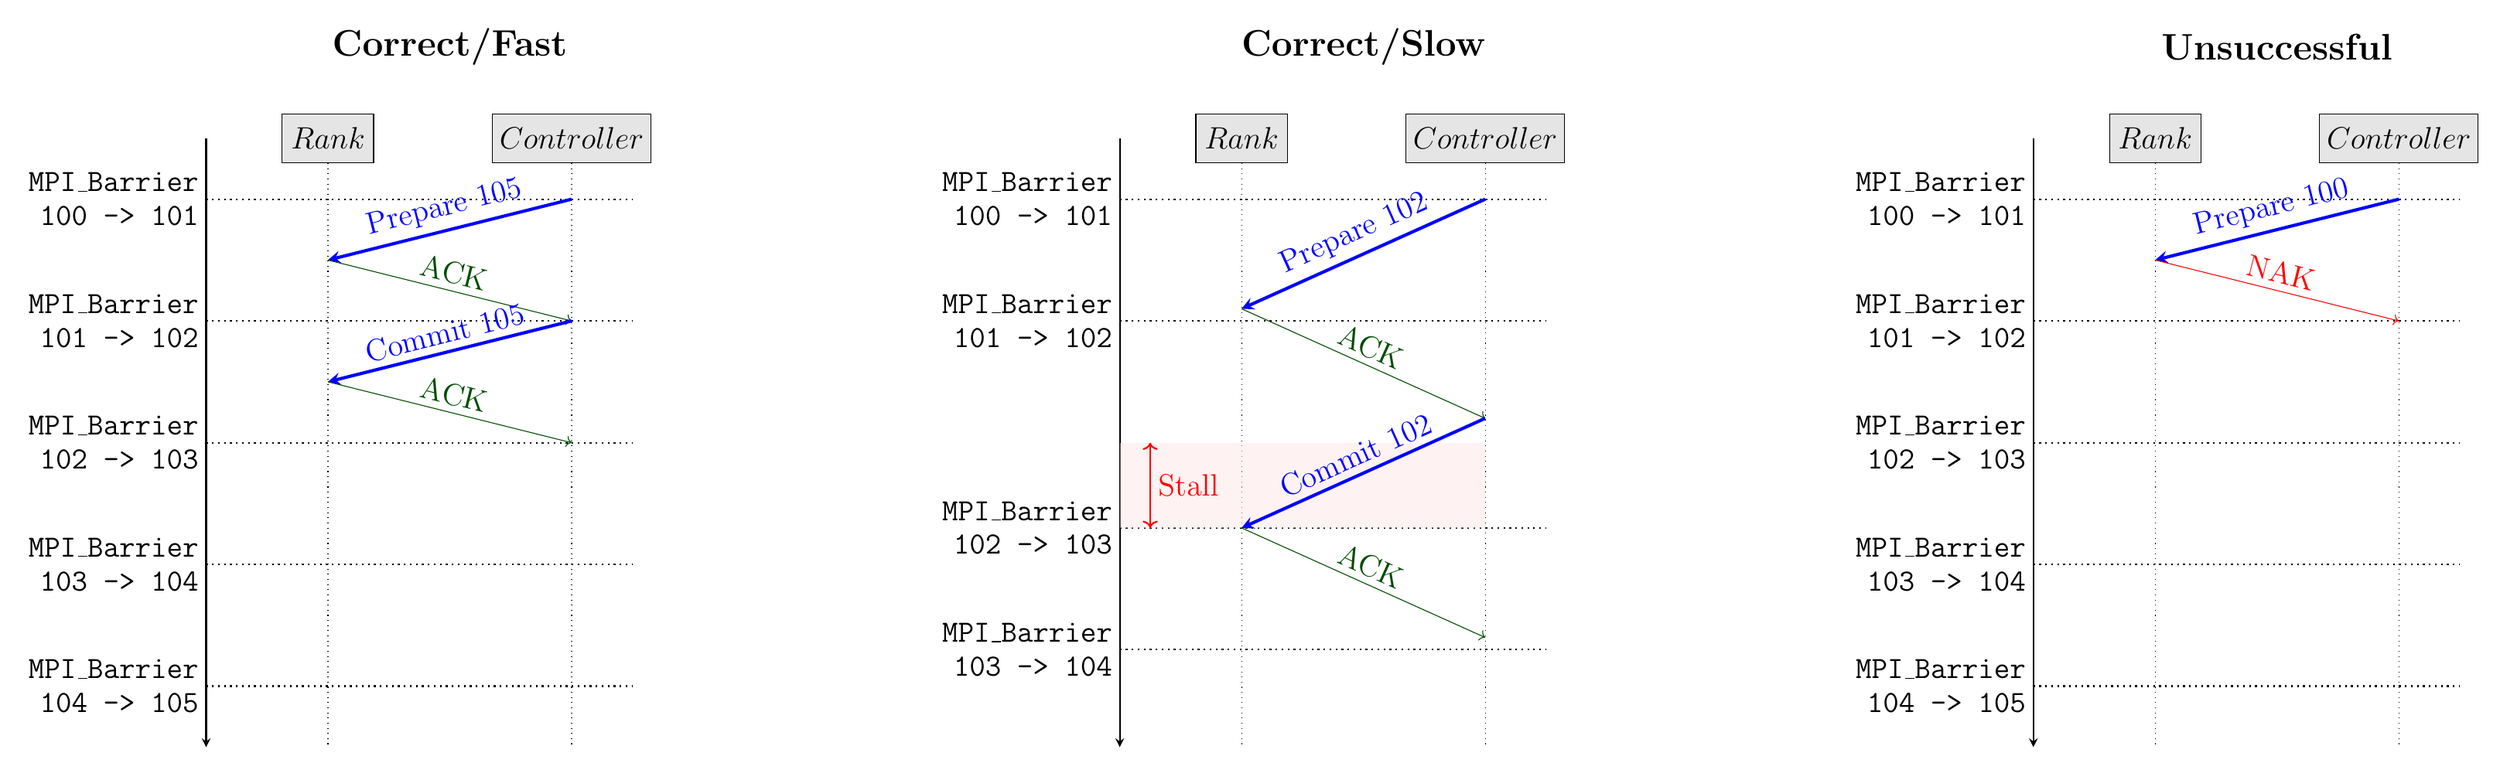
\begin{tikzpicture}[
  rankbox/.style={rectangle, draw, minimum width=1.5cm, minimum height=0.8cm, fill=gray!20},
  thread/.style={dotted, thick},
  font=\Large
  ] % temporary, to visualize grid
  % \draw[step=1cm, gray!10, very thin] (-4, -10) grid (10, 4);

  % annotate (0,0)
  % \node[anchor=north east] at (0,0) {(0, 0)};

  %% Common-case 2PC, non-blocking

  \begin{scope}[shift={(0, 0)}]
    \node[font={\LARGE\bfseries}] at (4, 1.5) {Correct/Fast};

    \rankcontroller

    % MPI barrier begin
    \tikzmath{%
      \step = -2;
      int \tsfrom;
      \tsfrom = 100;
      int \tsto;
      \yinit = -1;
      \xinit = 0;
      for \y in {0, 1, 2, 3, 4}{%
        \ypos = \yinit + \step * \y;
        \tsto = \tsfrom + 1;
        \yinit = -1;
        {
          \coordinate (c) at (\xinit, \ypos);
          \draw[style=thick,dotted] (c) -| ++(co) -- ++(1, 0);
          \node[anchor=south east] at (c) {\texttt{MPI\_Barrier}};
          \node[anchor=north east] at (c) {\texttt{{\tsfrom} -> \tsto}};
        };
        \tsfrom = \tsfrom + 1;
      };
      % MPI Barrier end
    }

  \end{scope}

  %% 

  \begin{scope}[shift={(15, 0)}]
    \node[font={\LARGE\bfseries}] at (4, 1.5) {Correct/Slow};

    \rankcontroller
    % MPI barrier begin
    \tikzmath{%
      \step = -2;
      int \tsfrom;
      \tsfrom = 100;
      int \tsto;
      \yinit = -1;
      \xinit = 0;
      for \ydel in {0, -2, -5.4, -7.4}{%
        \ypos = \yinit + \ydel;
        \tsto = \tsfrom + 1;
        \yinit = -1;
        {
          \coordinate (c) at (\xinit, \ypos);
          \draw[style=thick,dotted] (c) -| ++(co) -- ++(1, 0);
          \node[anchor=south east] at (c) {\texttt{MPI\_Barrier}};
          \node[anchor=north east] at (c) {\texttt{{\tsfrom} -> \tsto}};
        };
        \tsfrom = \tsfrom + 1;
      };
    }
    % MPI Barrier end
  \end{scope}

  \begin{scope}[shift={(30, 0)}]
    \node[font={\LARGE\bfseries}] at (4, 1.5) {Unsuccessful};

    \rankcontroller
    % MPI barrier begin
    \tikzmath{%
      \step = -2;
      int \tsfrom;
      \tsfrom = 100;
      int \tsto;
      \yinit = -1;
      \xinit = 0;
      for \y in {0, 1, ..., 4}{%
        \ypos = \yinit + \step * \y;
        \tsto = \tsfrom + 1;
        \yinit = -1;
        {
          \coordinate (c) at (\xinit, \ypos);
          \draw[style=thick,dotted] (c) -| ++(co) -- ++(1, 0);
          \node[anchor=south east] at (c) {\texttt{MPI\_Barrier}};
          \node[anchor=north east] at (c) {\texttt{{\tsfrom} -> \tsto}};
        };
        \tsfrom = \tsfrom + 1;
      };
    }
    % MPI Barrier end
  \end{scope}

  % Two-phase commit begin
  \tikzmath{%
    \xcont = 6;
    \xrank = 2;
    \yfrom = -1;
    \msgdelta = -1;
    \yto = \yfrom + \msgdelta;
    {
      \draw[->, line width=1.5pt, >=stealth, style=blue] 
      (\xcont, \yfrom) -- (\xrank, \yto)
      node[midway, above, sloped]{Prepare 105};
    };
    \yfrom = \yto;
    \yto = \yfrom + \msgdelta;
    {
      \draw[->,color=green!30!black] (\xrank, \yfrom) -- (\xcont, \yto)
      node[midway, above, sloped]{ACK};
    };
    \yfrom = \yto;
    \yto = \yfrom + \msgdelta;
    {
      \draw[->, line width=1.5pt, >=stealth, style=blue] 
      (\xcont, \yfrom) -- (\xrank, \yto)
      node[midway, above, sloped]{Commit 105};
    };
    \yfrom = \yto;
    \yto = \yfrom + \msgdelta;
    {
      \draw[->,color=green!30!black] (\xrank, \yfrom) -- (\xcont, \yto)
      node[midway, above, sloped]{ACK};
    };
  }
  % Two-phase commit end

  %% Stall box
  \filldraw[fill=red!10, fill opacity=0.5, draw=none] 
  (15, -5) rectangle (21, -6.4);

  \draw[<->, thick, draw=red] (15.5, -5) -- (15.5, -6.4)
  node[midway, right, text=red] {Stall};


  % Stalled Two-phase commit begin
  \tikzmath{%
    \xcont = 21; % controller x
    \xrank = 17; % rank x
    \yfrom = -1;
    \msgdelta = -1.8;
    \yto = \yfrom + \msgdelta;
    {
      \draw[->, line width=1.5pt, >=stealth, style=blue] 
      (\xcont, \yfrom) -- (\xrank, \yto)
      node[midway, above, sloped]{Prepare 102};
    };
    \yfrom = \yto;
    \yto = \yfrom + \msgdelta;
    {
      \draw[->, color=green!30!black] (\xrank, \yfrom) -- (\xcont, \yto)
      node[midway, above, sloped]{ACK};
    };
    \yfrom = \yto;
    \yto = \yfrom + \msgdelta;
    {
      \draw[->, line width=1.5pt, >=stealth, style=blue] 
      (\xcont, \yfrom) -- (\xrank, \yto)
      node[midway, above, sloped]{Commit 102};
    };
    \yfrom = \yto;
    \yto = \yfrom + \msgdelta;
    {
      \draw[->,color=green!30!black] (\xrank, \yfrom) -- (\xcont, \yto)
      node[midway, above, sloped]{ACK};
    };
  }
  % Two-phase commit end

  % Rejected Two-phase commit begin
  \tikzmath{%
    \xcont = 36; % controller x
    \xrank = 32; % rank x
    \yfrom = -1;
    \msgdelta = -1;
    \yto = \yfrom + \msgdelta;
    {
      \draw[->, line width=1.5pt, >=stealth, style=blue] 
      (\xcont, \yfrom) -- (\xrank, \yto)
      node[midway, above, sloped]{Prepare 100};
    };
    \yfrom = \yto;
    \yto = \yfrom + \msgdelta;
    {
      \draw[->,red] (\xrank, \yfrom) -- (\xcont, \yto)
      node[midway, above, sloped]{NAK};
    };
  }
  % Two-phase commit end

\end{tikzpicture}
\end{document}

